%\input{myformulae.tex}


\section{Preliminaries}

\subsection{FSM model for sequential circuits}
A finite state machine (FSM) is a mathematical model of computation for designing and analyzing sequential logic 
circuits. If a FSM's primary outputs depend on primary inputs and present state inputs, it is named as a \textit{Mealy machine};
the formal definition is as follows:
\begin{definition}
A Mealy machine is an $n$-tuple $\mathcal M = (\Sigma,O,S,S^0,\Delta,\Lambda)$ where
\begin{itemize}
\item $\Sigma$ is the input label, $O$ is the output label;
\item $S$ is the set of states, $S^0\subseteq S$ is the set of initial states;
\item $\Delta:\ S\times\Sigma\to S$ is the next state transition function;
\item $\Lambda:\ S\times\Sigma\to O$ is the output function.
\end{itemize}
\end{definition}
The other kind of FSM is \textit{Moore machine}, its difference from Mealy machine is that
its primary outputs only depend on the present states, i.e. the output function is defined as
$$\Lambda:\ S \to O$$
Typical sequential circuits can be depicted as Fig.\ref{fig:seqmodel}(a). Primary inputs
$x_1,\dots,x_m \in \Sigma$, and primary outputs $z_1,\dots,z_n\in O$. Signals $s_1,\dots,s_k$ 
are present state (PS) variables, $t_1,\dots,t_k$ are next state (NS) variables.
We can define 2 $k$-bit words denoting the PS/NS variables as there are $k$ flip-flops
in the datapath: $S = (s_1,\dots,s_k), ~T=(t_1,\dots,t_k)$. Transition function
at bit level are defined as $\Delta_i: t_i = \Delta_i(s_1,\dots,s_k,x_1,\dots,x_m)$.
\begin{figure}[hbt]
\centering{
%\begin{minipage}{12cm}
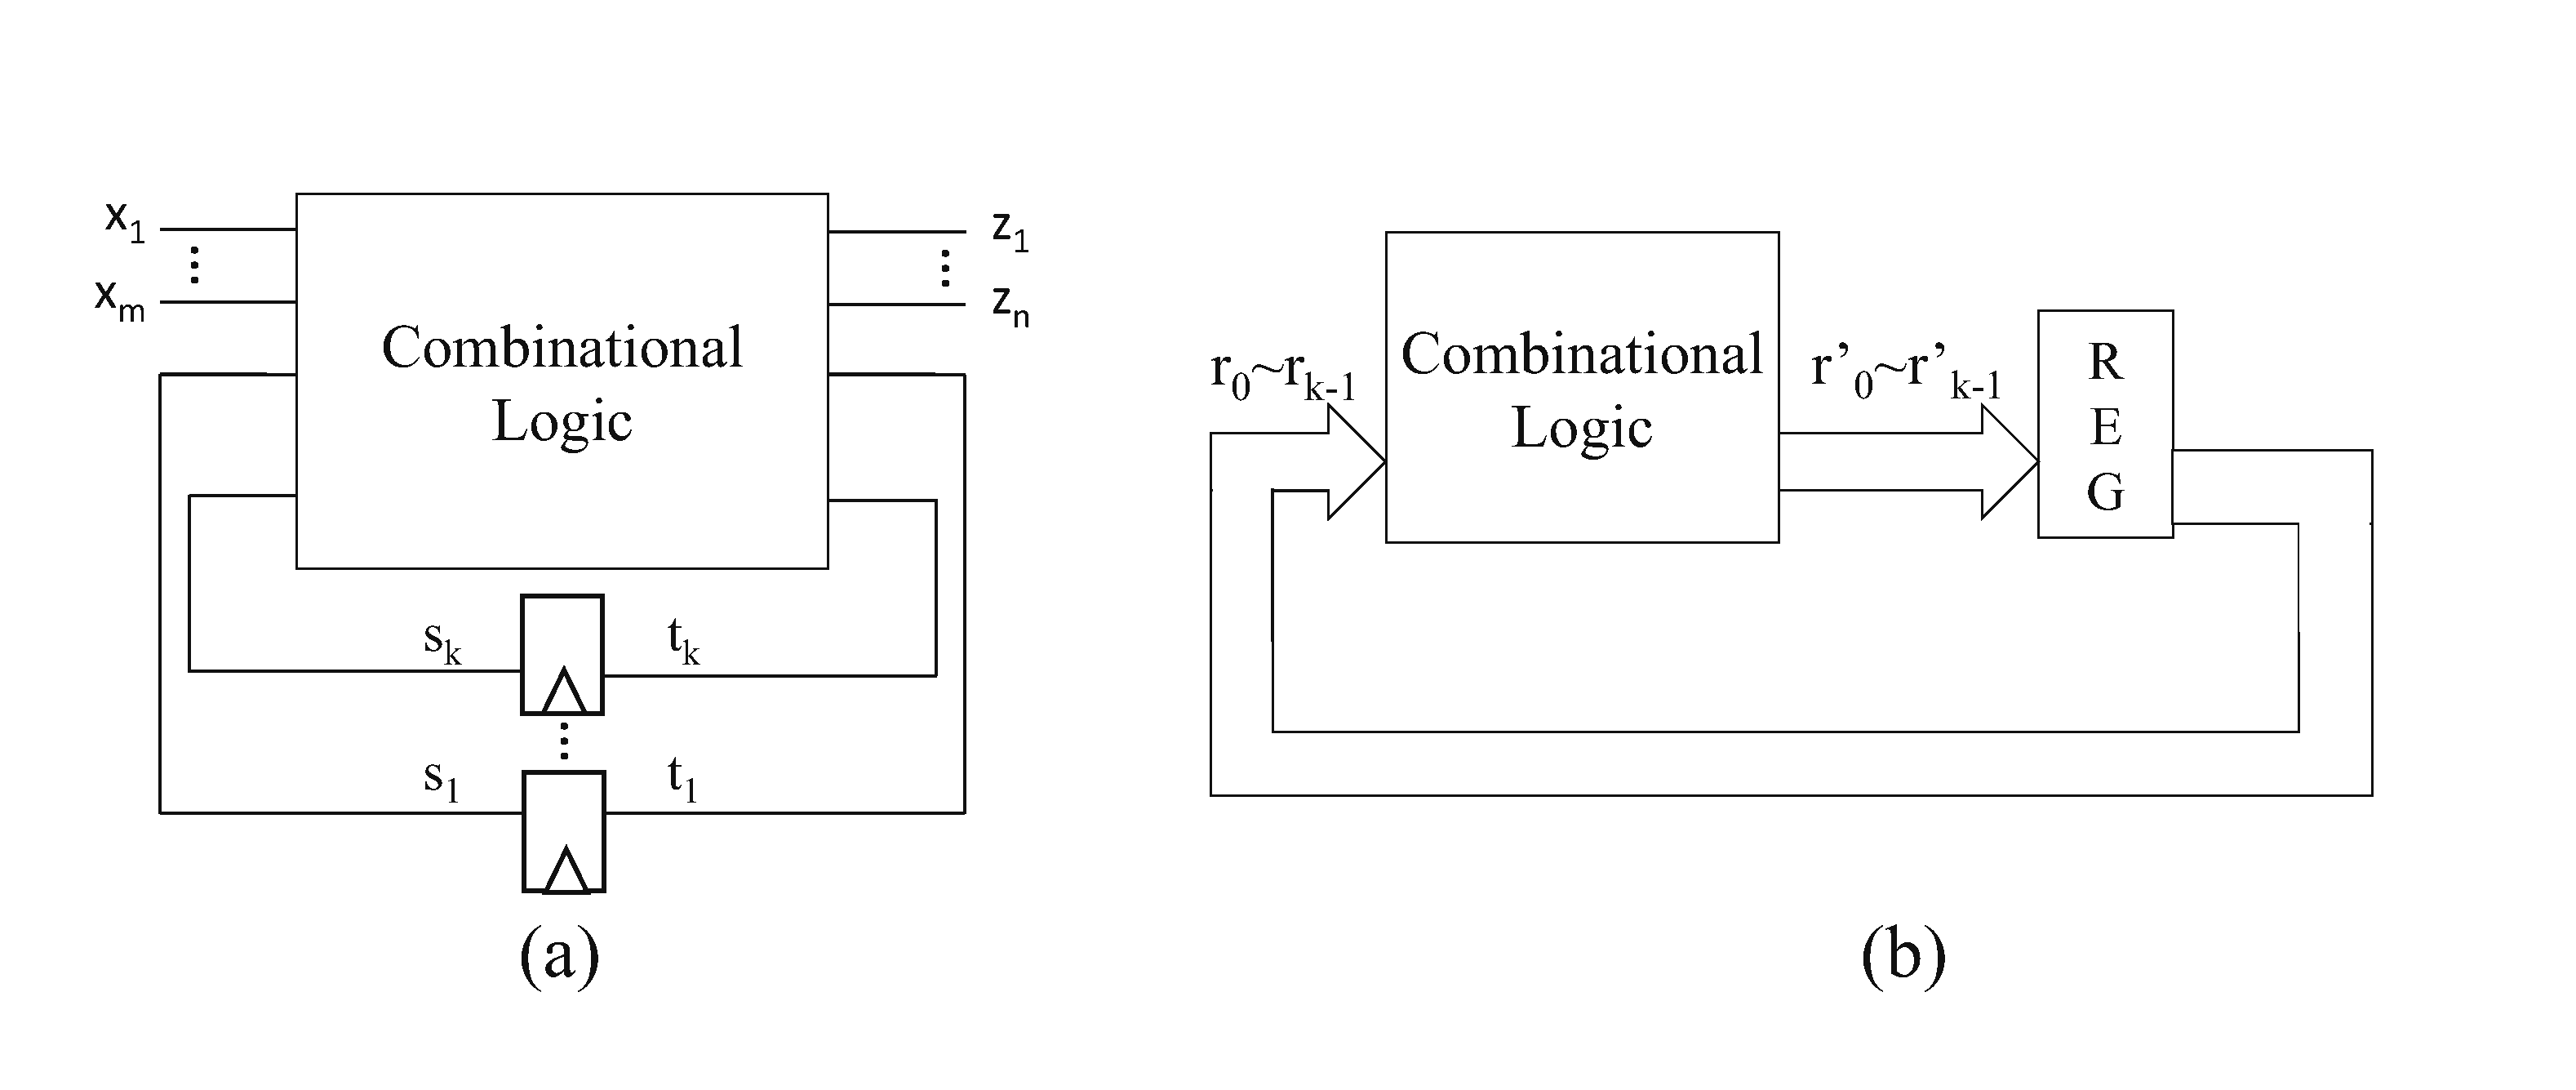
\includegraphics[width=5.5in]{./seqmodel.eps}
% \vspace{-0.2in}
\caption{FSM models of sequential circuits}
%\end{minipage}
\label{fig:seqmodel}}
\end{figure}
In some cases, arithmetic computations are implemented as Moore machines where input operands
are loaded into register files $R$ and the FSM is executed for $k$ clock cycles.
We can simplify them to the model in Fig.\ref{fig:seqmodel}(b).

\subsection{Commutative algebra and algebraic geometry preliminaries}
A {\bf field} $\mathbb{F}$ is a set of elements, including 0 and 1 (unity),
allowing for associative and commutative addition and multiplication;
and every non-zero element has a multiplicative inverse.  A {\bf
  finite field} or {\bf Galois filed} is a field with a finite number
($q$) of elements, and is denoted by $\Fq$, where $q=p^k$ is a power of
a prime integer $p$. In our work, $q = 2^k$ for
a given $k$, where $k$ represents the datapath (bit-vector)
word-lengths, or the number of memory elements (state registers) in
finite state machines. 

Let the field $\mathbb{F}_2 = \{0, 1\} ~(\equiv \B)$, and let
$\mathbb{F}_2[X]$ denote the set (ring) of all univariate polynomials
in variable $X$ with coefficients from $\mathbb{F}_2$. Then, the
Galois field $\Fkk$ is constructed as $\Fkk = \mathbb{F}_2[X] \pmod{
  P(X)}$, where $P(X)$ is an irreducible polynomial over
$\mathbb{F}_2$. Let $\alpha$ be a root of the irreducible polynomial
$P(X)$, i.e. $P(\alpha) = 0$. Any element $A \in \Fkk$ can be
represented as $A = \sum_{i=0}^{k-1} a_i \alpha^i$, where $a_i \in
\mathbb{F}_2$. The field $\Fkk$ is therefore, a $k$-dimensional {\it
  extension} of the base field $\mathbb{F}_2$: so,  $\mathbf{\Fkk \supset
\mathbb{F}_2}$. Consequently, all operations of addition and
multiplication in $\Fkk$ are performed modulo the irreducible
polynomial $P(\alpha)$ and coefficients are reduced modulo 2.  

Boolean variables in field $\mathbb B$ can be easily mapped to
elements in $\mathbb F_2$. Since $\mathbb F_2 \subset \Fkk$, these 
%Namely $k$-bit Boolean bit-vector defined
%over Boolean ring $\mathbb B^k$ can also be mapped uniquely  to $\Fkk
%= \mathbb F_2[x_1,\dots,x_k]$. 
Boolean operators are interpreted as functions over $\Fkk$ (where $+$
and $\cdot$ are addition and multiplication performed modulo 2): 
\begin{align*}
&a\land b \to a\cdot b\\
&a\oplus b \to a+b\\
&\neg a \to 1+a\\
&a \bar{\oplus} b \to 1+a+b\\
&a \lor b \to a+b+a\cdot b
\end{align*}

Using these mappings we can write Boolean functions in form of
polynomials over $\mathbb F_2\subset \Fkk$. 
These concepts provide a mechanism to represent and
manipulate both bit-level ($\mathbb{F}_2$) and $k$-bit word-level
constraints {\bf in one unified mathematical domain $\Fkk$ --- a
  concept we   exploit for abstraction. }
  Consider Ex.\ref{ex:motiv},
polynomials for transition functions (bit-level outputs) $f_1,f_2$
are over $\mathbb F_2$, i.e. $f_1,f_2\subseteq \mathbb F_2 \subset \Fkk$,
and polynomials containing word-level variables $f_3,f_4,f_5 \subseteq \Fkk$.
All polynomials belong to unified domain $f_1,f_2,\dots,f_5 \subseteq \Fkk$.

It is well-known that every Boolean mapping between $k$ dimensional
Boolean spaces $f: \B^k \rightarrow \B^k$ can be construed as a
function over Galois fields $f: \Fkk \rightarrow \Fkk$. Moreover,
every function $f: \Fkk \rightarrow \Fkk$ is a polynomial function: 
i.e. $f$ can be represented by way of a unique, minimal, canonical
polynomial $\F(X)$, and the work of \cite{timDAC} shows how to
efficiently derive such polynomial representations from circuits ---
another concept that makes our approach feasible. 


We represent Boolean circuits by way of polynomials over
$\Fkk$. If we take indeterminates $x_1,x_2,\dots,x_n$, an arbitrary
combination of their finite product  
$x_1^{d_1}\cdot x_2^{d_2}\cdots x_n^{d_n}, d_i\geq 0$ 
is a {\bf monomial}. A {\bf polynomial} $f = c_1 X_1 + c_2 X_2 + \dots
+ c_t X_t$ is a finite sum of terms, where $c_1, \dots, c_t$ are
coefficients and $X_1, \dots, X_t$ are monomials. The set of {\it all}
such polynomials with coefficients from $\Fkk$ forms a {\bf
  multivariate polynomial ring} denoted $\Fkk[x_1,\dots,x_n]$. 
A monomial ordering $X_1 > X_2 \dots > X_t$ is imposed on the
polynomials to process them systematically. Then, $LT(f) = c_1 X_1,
LM(f) = X_1$ denote the leading term and the leading monomial of $f$,
respectively. 


Multivariate polynomial division will play a key role in our
algorithmic techniques. Division is implemented as {\it cancellation
  of terms.} Given polynomials $f, g$, if $cX$ is a term in
$f$ that is divisible by $LT(g)$, then $f \xrightarrow{g} r$ denotes a
one-step reduction (division) of $f$ by $g$, resulting in remainder $r
= f - {{cX} \over {LT(g)}} \cdot g$. This has the effect of cancelling
the term $cX$ from $f$. 
\begin{example}
\label{ex:multidiv}
If $f = e + cd$ and $g = c + ab$,
then the term $cd$ in $f$ can be canceled by $LT(g) = c$: $r = f - {cd
  \over c} g = e + abd$. 
\end{example}
  Similarly, $f$ reduces to $r$ modulo the set
of polynomials $F = \{f_1, \dots, f_s\}$, denoted $f \stackrel{F}
{\textstyle   \longrightarrow}_+ r$, such that no term in $r$ is
divisible (cancellable) by the $LT(f_i)$ of any polynomial in $ f_i
\in F$.    


In verification, we have to analyze the {\it solutions to a
set of polynomials.} The set of all solutions to a system of
polynomial equations $f_1 = \dots = f_s = 0$ is defined as the affine variety:
\begin{definition}
Given a set of polynomials $f_1,\dots,f_s$ over ring $\mathbb F_q[x_1,\dots,x_n]$, their 
{\bf affine variety} 
$$V(f_1,\dots,f_s) = \{(a_1,\dots,a_n)\in  (\mathbb F_q)^n |
f_1(a_1,\dots,a_n) = \cdots = f_s(a_1,\dots,a_n) = 0\}$$ 
\end{definition}

Generally we can find many sets of polynomials with the same variety, which are linear combinations
of given set of polynomials. This set is defined as follows:
\begin{definition}
{\bf Ideal of Polynomials:} Let $f_1,f_2,\dots,f_s\in \mathbb F[x_1,\dots,x_n]$.
Define an ideal
$$J = \langle f_1,f_2,\dots,f_s\rangle = \{f_1\cdot h_1 + f_2\cdot h_2 +\cdots + f_s\cdot h_s : h_1,\dots,h_s\in \mathbb F[x_1,\dots,x_n]\}$$
We call $J = \langle f_1,f_2,\dots,f_s\rangle$ an ideal generated by $f_1,\dots,f_s$ and these polynomials 
the {\bf generators} of ideal $J$.
\end{definition}
% On the other hand, if given another polynomial $f$, we need to judge whether it belongs to $J$.
A practical problem is: given an ideal $J = \langle f_1,f_2,\dots,f_s\rangle$ and a polynomial $f$,
we need to check if the variety of $J$ can make the evaluation of $f$ equal to 0, i.e. $f$ vanishes on $V(J)$.
This problem is usually described as ideal membership checking problem.
\begin{definition}
{\bf Ideal membership:} Let $f_1,f_2,\dots,f_s\in \mathbb F[x_1,\dots,x_n]$, and $J = \langle f_1,f_2,\dots,f_s\rangle$
be an ideal over ring $\mathbb F[x_1,\dots,x_n]$. If 
$$f = f_1h_1 + f_2h_2 + \cdots + f_sh_s$$
then $f\in J$.
\end{definition}

An ideal may have many generating sets. For example, we may have different set of polynomial generators denoting
the same ideal, where they have the same variety: $\langle f_1,\dots,f_s\rangle = \langle h_1,\dots,h_r\rangle
= \langle g_1,\dots,g_t\rangle$ such that $V(f_1,\dots,f_s) = V(h_1,\dots,h_r) = V(g_1,\dots,g_t)$.
Therefore a canonical representation of an ideal is needed, which leads to the concept of Gr\"obner bases.

\begin{definition}
The set $G = \{g_1, \dots,
g_t\}$ is called a \textbf{\Grobner basis} of $J$ if and only if the
leading term of all polynomials in $J$ is divisible be the leading
term of some polynomial $g_i$ in $G$: i.e. $\forall f \in J, \exists
g_i \in G \ s.t. \ LT(g_i) ~|~ LT(f)$. 
\end{definition}
% The famous Buchberger's
% algorithm, given in textbook \cite{ideals:book}, is used to compute a
% \Grobner basis (GB). Operating on  input $F = \{f_1, \dots, f_s\}$,
% and subject to the imposed term order $>$, it derives $G = GB(J) = \{
% g_1, \dots, g_t \}$. Buchberger's algorithm repeatedly computes
% $S$-polynomials. For pairs $(f_i, f_j) \in F$, $Spoly(f_i, f_j) =
% \frac{L}{lt(f_i)}\cdot f_i - \frac{L}{lt(f_j)}\cdot f_j$, where $L =
% LCM(LM(f_i), LM(f_j))$. Reducing $Spoly(f_i, f_j) \xrightarrow{F}_+ r$
% cancels the leading terms of $f_i, f_j$ and gives a polynomial $r$
% with a new leading term. This remainder $r$ is added to the current
% basis and $Spoly(f_i, f_j)$ computations are repeated for all pairs of
% polynomials until all $S$-polynomials reduce to 0.  

An advantage of representing an ideal with GB is that it can serve as a decision procedure for ideal membership
test when dividing a polynomial $f$ by a GB, i.e.
$$G = GB(J) \Longleftrightarrow \forall f\in J, f\xrightarrow{g_1,g_2,\dots,g_t}_{+} 0$$
Gr\"obner basis can be reduced by eliminating redundant elements. \textbf{A reduced GB is a canonical representation of 
the ideal under a given monomial ordering}. Given an ideal $J = \langle f_1,\dots,f_s\rangle, ~G = 
\{g_1,\dots,g_t\}$ is the GB of $J$, it can be computed by Buchberger's algorithm (refer to textbook \cite{ideal:book}).

Another advantage of using GB representation is that GB computation can work as a {\it quantification procedure}.
In the following part we will introduce the concept of \textit{vanishing polynomials}, \textit{elimination ideal}, etc.
as the bases of this theory.

{\it Fermat's little theorem over $\Fq$:} For any $ \alpha \in \mathbb
F_{q}, \alpha^q = \alpha$. Therefore, the polynomial $x^q - x$
vanishes ($=0$) over $\Fq$, and is called a vanishing polynomial. We
denote by $J_0 = \langle x_1^q - x_1, \dots, x_d^q - x_d \rangle$ the
ideal of all vanishing polynomials in $\Fq[x_1, \dots, x_d]$. When $q
= 2^k, x^q - x = x^q + x$ as $-1 = +1$ over $\Fkk$.

Gr\"obner bases can be used to {\it eliminate} (i.e. quantify) variables from an
ideal. Given ideal $J = \langle f_1,\dots,f_s\rangle \subset \mathbb
F_{q}[x_1,\dots,x_d]$, the $l^{th}$ elimination ideal $J_l$ is the
ideal of $\Fq[x_{l+1}, \dots, x_d]$ defined by $J_l = J \cap
\Fq[x_{l+1}, \dots, x_d]$. Variable elimination can be achieved 
by computing a Gr\"obner basis of $J$ w.r.t. elimination orders: 
\begin{theorem}
\label{thm:elim}
(Elimination theorem\cite{ideals:book}) Let $J\subset \mathbb
  F_{2^k}[x_1,\dots,x_d]$ be an ideal and let $G$ be a Gr\"obner basis
  of $J$ with respect to a lexicographic (LEX) ordering where
  $x_1>x_2>\cdots>x_d$. Then for every $0\leq l\leq d$, the set $G_l =
  G\cap\mathbb F_{2^k}[x_{l+1},\dots,x_d]$ is a Gr\"obner basis of
  the $l$-th elimination ideal $J_l$.
\end{theorem}
We describe an application of elimination ideals using following example borrowed from \cite{ideals:book}:
\begin{example}
Consider polynomials $f_1: x^2-y-z-1;\ f_2:x-y^2-z-1;\ f_3:x-y-z^2-1$ and ideal $J = \langle f_1,f_2,f_3\rangle
\subset \mathbb C[x,y,z]$. Gr\"obner basis $G = GB(J)$ w.r.t. LEX term order equals to 
$g_1:x-y-z^2-1;\ g_2:y^2-y-z^2-z;\ g_3: 2yz^2-z^4-z^2;\ g_4:z^6-4z^4-4z^3-z^2$. From observation,
we find that the polynomial $g_4$ only contains variable $z$ ($x,y$ eliminated), and polynomials $g_2,g_3,g_4$ only contain variables
$y,z$ ($x$ eliminated). According to theorem \ref{thm:elim}, $G_1 = G\cap\mathbb C[y,z] = \{g_2,g_3,g_4\}$
is the Gr\"obner basis of the $1^{st}$ elimination ideal of $J$ and $G_2 = G\cap\mathbb C[z] = \{g_4\}$ is the 
$2^{nd}$ elimination ideal of $J$, respectively.
\end{example}

\subsection{Application of elimination theorem on circuit verification}
\label{sec:elim}
Assume that we are given a circuit (combinational component) with input $A = (a_0,\dots,a_{k-1})$ and output 
$R = (r_0,\dots,r_{k-1})$ (both can be represented
by word level variables in $\Fkk$). We can describe this circuit with an elimination ideal $J+J_0$, where
$J$ is the ideal generated by the polynomials corresponding to circuit gates and $J_0$ is the ideal of vanishing polynomials.
The authors of \cite{timDAC} showed that for any combinational
logic block, a canonical word-level polynomial representation can be
derived through \Grobner bases computed with elimination orders:
\begin{lemma}
(From \cite{timDAC}) Given a combinational circuit $C$ with $k$-bit
  input $A = (a_0, \dots, a_{k-1})$ and $k$-bit output $R = (r_0, \dots,
  r_{k-1})$. Denote by $x_1, \dots, x_d$ all the bit-level
  variables of   $C$. Let $J = \langle f_1, \dots, f_s \rangle \subset
  \Fkk[x_1, \dots, x_d, R, A]$ denote all the polynomials corresponding to the
  logic gates of the circuit. Let $J_0 = \langle x_1^2 - x_1, \dots,
  x_d^2 - x_d, R^q - R, A^q - A \rangle$ be the vanishing ideal, so
  that $J + J_0 = \langle f_1, \dots, f_s, ~~ x_1^2 - x_1, \dots,
  x_d^2 - x_d, R^q - R, A^q - A \rangle$. Compute \Grobner basis $G =
  GB(J + J_0)$ w.r.t. lex term order with $x_1 > x_2 > \dots > x_d > R
  > A$. Then $G_d = G \cap \Fkk[R, A]$ eliminates the internal
  variables $x_1, \dots, x_d$ of the circuit. $G_d$ also contains the
  word-level polynomial $R = \F(A)$ which canonically represents the
  function of the circuit with only word level variables $R$ and $A$.
\end{lemma}
This lemma shows an application of GB computations over an elimination ideal.
Since it abstracts the function of a combinational circuit, we call the term order
$primary~inputs~and~intermediate~variables~>~word~level~output~>~word~level~inputs$
as \textit{abstraction term order} (ATO).
If we further eliminate word-level input, the result will be a polynomial containing only 
the word-level output variable. In a sequential circuit
such as Ex.\ref{ex:motiv}, the output of combinational logic serves as the next state variable. Polynomial $g_T$ in
the example is the desired projection; i.e. using GB computation on elimination ideal and eliminating to NS
variables provides us the canonical representation of reachable states in next time frame.



% Machine traversal is key for many verification techniques, e.g. to check
% the equivalence of 2 FSMs, we can observe whether the output responses are the same at
% every step of traversal. An explicit traversal is usually infeasible, here we use 
% implicit state enumeration (BFS traversal) based on Boolean formulas to implement a machine traversal.
% The algorithm is as follows:
% \begin{algorithm}[hbt]
% \SetAlgoNoLine
%  \KwIn{Transition functions $\Delta$, initial state $S^0$}
% 
%   $from^0 = reached = S^0$\;
%   \Repeat{$new^i == 0$}
%   {
%   	$i \gets i + 1$\;
% 	$to^i \gets$Img$(\Delta, from^{i-1})$\;
% 	$new^i \gets to^i \cap \overline{reached}$\;
%   	$reached \gets reached \cup new^i$\;
% 	$from^i \gets new^i$\;
%   }
% \Return{$reached$}
% \caption {Breadth-first Traversal Algorithm for Reachability Analysis of FSMs}\label{alg:BFS}
% \end{algorithm}
% The main computation in this algorithm is the \textit{image function}. Img$(\Delta,from^{i-1})$
% denotes the forward image of the set $from^{i-1}$ under the transition function $\Delta$.
% Let  $\Delta_i$ denote the transition relation 
% for $i^{th}$ bit of output $T$ (denoted by $t_i$), and it is described by a Boolean function. We can obtain the transition relation 
% for bit-vector $T$: $Tran(s_0,s_1,x,t_0,t_1) = \bigwedge_{i=1}^{2}(t_i\ \bar{\oplus}\ \Delta_i)$. Assume present states
% are represent by Boolean formulas $PS(s_0,s_1)$, then the image function is written as
% $\text{Img}(Tran,\ PS) = \exists_{s_0,s_1}\exists_{x}[Tran(s_0,s_1,x,t_0,t_1)\land PS(s_0,s_1)]$, where
% $\exists_x f$ denotes the existential quantification of $f$ w.r.t. $x$.
% \begin{example}
% We use implicit state enumeration based on Boolean formulas to traverse FSM in Fig.\ref{fig:fsm}.
% Initial state $\{00\}$ can be represented by Boolean formula $C(s) = \overline{s_0}\cdot \overline{s_1}$.
% Transition function for $NS$ variables are 
% $$t_0\overline{\oplus}\Delta_0 = t_0\overline{\oplus}(\overline{x}\overline{s_0}\overline{s_1}+s_0s_1)$$
% $$t_1\overline{\oplus}\Delta_1 = t_1\overline{\oplus}(x\overline{s_0}+s_0\overline{s_1})$$
% \end{example}